\documentclass[journal,twoside,web]{ieeecolor}
\usepackage{jsen}
\usepackage{cite}
\usepackage{amsmath,amssymb,amsfonts}
\usepackage{algorithmic}
\usepackage{graphicx}
\usepackage{textcomp}
\usepackage{wrapfig}
\usepackage{url}

\graphicspath{ {./images/} }
\def\BibTeX{{\rm B\kern-.05em{\sc i\kern-.025em b}\kern-.08em
    T\kern-.1667em\lower.7ex\hbox{E}\kern-.125emX}}
\markboth{Spring 2020}
{Pathan Faisal Khan: Big Data Analytics}

\begin{document}
\title{Using Apache Spark to predict finish placement in PlayerUnknown’s Battlegrounds game}
\author{Pathan Faisal Khan, Letterkenny Institute of Technology
\thanks{Under the supervision of Dr. Shagufta Henna, Letterkenny Institute of Technology, Letterkenny, CO. Donegal}
}

\IEEEtitleabstractindextext{
\begin{abstract}

\end{abstract}

\begin{IEEEkeywords}

\end{IEEEkeywords}}

\maketitle

\section{Introduction}
\label{sec:introduction}
\IEEEPARstart{P}{layerUnknown's} Battlegrounds (PUBG)~\cite{noauthor_playerunknowns_nodate} is an online shooter multiplayer game of battle royale genre~\cite{noauthor_battle_2019} inspired by the Japanese film "Battle Royale"~\cite{fukasaku_battle_2000}. The game is playable on Personal Computers (PC), Sony's PlayStation, Micorsoft's Xbox and mobile devices (Android and iOS). It was developed and published in late 2017 by South Korean video game company Bluehole's subsidiary PUBG Corporation. Since it's launch, PUBG has seen exponential growth. It crossed the 1 million players mark within 48 hours of its release on consoles and a total of 30 million copies were sold for both PC and consoles just within a few days of its release. It has gained quite a good traction in Asian countries especially in China and India on to its mobile version with India standing at 116 million downloads which makes 21\% of its total worldwide downloads followed by China with 108 million downloads which accounted for 19\% while the USA stood at 8\% with 42 million downloads~\cite{mcaloon_now_nodate}. With these many players on its platform, it generated vast amounts of data.

The game's most popular mode, classic mode, allows up to 100 players to parachute on an area of up to 8 x 8 kilometers island on which players will fight with each other in teams of maximum 4 players, the team to survive at the last is winner. The game world depending on the map selected has different terrains with sea, rivers, deserts, forests, snow, roads and bridges. Buildings and towns are spread across the map which has weapons and other essential items for a player to fight and survive in the game.

This technical report is going to explore a publicly available dataset~\cite{noauthor_pubg_nodate} of the popular game. At the time of writing this report, the dataset is hosted on a popular online community for data scientists and machine learning practitioners, Kaggle~\cite{noauthor_kaggle_nodate}. The code for this report has been open-sourced and hosted on Github~\cite{khan_faisal3325/pubg_prediction_2020}.

\textbf{The data} is taken from Kaggle's competition on "PUBG Finish Placement Prediction"~\cite{noauthor_pubg_nodate}. It contains data of 65,000 matches where each row defines a player's stats after they finish their game. The training set has 4,446,966 rows while the testing set has 1,934,174 rows and 29 variables. The data is complete, but it requires some pre-processing for converting categorical variables to numerical.

\textbf{The primary goal of this technical report} is predicting percentile of a player's finishing position where 0 denotes last position and 1 stands for 1st position in a match. The report has also answered the following questions with visualizations based on analysis of the data:
\begin{enumerate}
    \item Average time a player spends in a match.
    \item Total number of kills done by users when playing alone versus when playing in a team.
    \item How better a player performs (in terms of rankPoints, winPlace, winPoints) when playing alone versus when playing in a team?
\end{enumerate}
All these computations will be performed on distributed computing framework due to large size of the data.

\textbf{Organization of the report} is formatted in the following way. The paper will start with a brief overview of the program paradigm in Section \textbf{\ref{sec:system_overivew}}. Later on, the algorithms used for prediction will be covered in Section \textbf{\ref{sec:algorithms}}. The implementation plan which describes the data pre-processing stage as well as model creation will be discussed in Section \textbf{\ref{sec:implementation}}. Section \textbf{\ref{sec:discussion}} will discuss the observations of the analysis answering the questions mentioned earlier. This section will also compare the used algorithms. The paper will finally conclude with the observations from this report in Section \textbf{\ref{sec:conclusion}}.

\section{System Overview}
\label{sec:system_overivew}
To run the algorithms, Apache Spark has been selected as the proposed solution which swiftly handles large datasets and computes parallely. Apache Sparks is used for performing large-scale data analytics using technologies used in modern data centers on the production level. Apache Spark will be implemented on a cloud solution. Google Cloud Platform (GCP) has been selected as the cloud service provider. Under GCP, the project will be implemented using Cloud Dataproc~\cite{noauthor_dataproc_nodate}, BigQuery~\cite{noauthor_bigquery_nodate} and Apache Spark's Machine Learning Library~\cite{noauthor_mllib_nodate}. With the combination of these services, we will be making out our analytics and prediction. Cloud Dataproc is described on the GCP website as " a fast, easy-to-use, fully managed cloud service for running Apache Spark and Apache Hadoop clusters in a simpler, more cost-efficient way"~\cite{noauthor_dataproc_nodate}. They have claimed that using their service, it has proven to reduce time consumption on operations which took hours or days on a traditional system to seconds or minutes~\cite{noauthor_dataproc_nodate}. BigQuery will be used in our project to store our datasets which provides a serverless and highly-scalable data warehousing solution. For implementing our model, we will be using Apache Spark's Machine Learning Library. The library is available in Java, Scala, and Python, we are interested to implement our model in Python. 

We will be creating jobs using Apache Spark ML library and running them on our Dataproc clusters. The Figure \ref{fig:1} shown below describes our expected workflow:

\begin{figure*}[]
  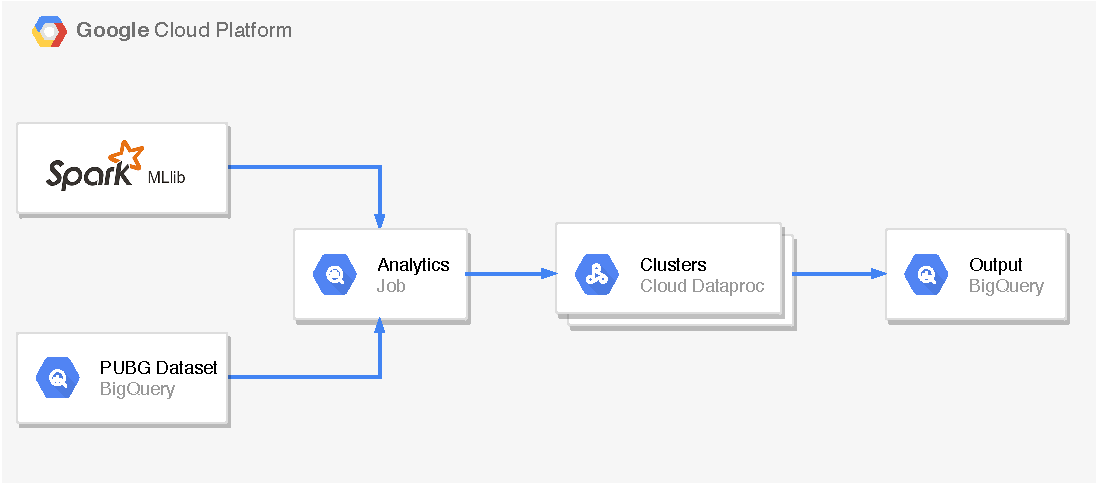
\includegraphics[width=\textwidth]{images/flow.pdf}
  \caption{Workflow of the analytics operation.}
  \label{fig:1}
\end{figure*}

\section{Algorithms}
\label{sec:algorithms}
Algorithms used in this report are for prediction of the win placement percentile of a given player. We have used regression algorithms, AdaBoost Regressor, Gradient Boosting Regressor, Random Forest Regressor and Decision Tree Regressor.

\subsection{AdaBoost Regressor}
AdaBoost, also known as Adaptive Boosting, is one of the first boosting algorithms proposed by Gödel Prize winners Robert E. Schapire and Yoav Freund in 2012 in their published book "Boosting: Foundations and Algorithms"~\cite{schapire_boosting_2012}. 

A boosting algorithm works by combining multiple weak algorithms which have no correlations amongst each other and voting for the best solution. In this way, a couple of weak algorithms come together to make one strong algorithm. Boosting algorithms are based on ensemble modelling, which literally means "a group producing a single effect".

AdaBoost uses decision tree with a single split as its weak algorithm often called as decision stumps and applies boosting over it. Since AdaBoost is based on ensemble modelling, it tries to fit all data points, it fails with noisy data. The most astonishing thing about this algorithm is that it does not overfits even though it is trying to fit all the data points. AdaBoost Regressor can be used both for classification and regression problems.

\subsection{Gradient Boosting Regressor}


\subsection{Random Forest Regressor}


\subsection{Decision Tree Regressor}
Decision tree is a predictive modelling algorithm which with the help of a collection of binary rules predict an output. These rules are formed by a QnA by the algorithm on the data to narrow down to the problem until it reaches a final conclusion. It can be used for both classification and regression problems. But this algorithm is not suitable for continuous variables and is also prone to over fitting.

\section{Implementation}
\label{sec:implementation}

\section{Experimentation Results and Discussions}
\label{sec:discussion}

\section{Conclusion}
\label{sec:conclusion}

\bibliographystyle{IEEEtran}
\bibliography{bib}

\end{document}
